\documentclass{beamer}

\usepackage{graphicx}
\usepackage{beamertexpower}
\usepackage{appendixnumberbeamer}
\usepackage[latin1]{inputenc}
\usepackage{pifont}
\usepackage{calc}
\usepackage{ae}
\usepackage{textcomp}
\usepackage{booktabs}
\usepackage{tabularx}
\usepackage{overpic}
\usepackage{animate}
\usepackage{tikz}
\usepackage{fixltx2e}

\usetikzlibrary{%
  arrows,%
  shapes,% 
  chains,%
  matrix,%
  positioning,% wg. " of "
  scopes,%
  %decorations.pathmorphing,% /pgf/decoration/random steps | erste Graphik
  shadows,%
  calc,
}

\newlength{\storage}
\newlength{\arrowwidth}
\makeatletter

% Document shape for tikz
\makeatletter
\newdimen\tempa
\newdimen\tempb
\pgfdeclareshape{doctype}{
    \inheritsavedanchors[from=rectangle]
    \inheritanchorborder[from=rectangle]
    \inheritanchor[from=rectangle]{north}
    \inheritanchor[from=rectangle]{north west}
    \inheritanchor[from=rectangle]{north east}
    \inheritanchor[from=rectangle]{center}
    \inheritanchor[from=rectangle]{west}
    \inheritanchor[from=rectangle]{east}
    \inheritanchor[from=rectangle]{mid}
    \inheritanchor[from=rectangle]{mid west}
    \inheritanchor[from=rectangle]{mid east}
    \inheritanchor[from=rectangle]{base}
    \inheritanchor[from=rectangle]{base west}
    \inheritanchor[from=rectangle]{base east}
    \inheritanchor[from=rectangle]{south}
    \inheritanchor[from=rectangle]{south west}
    \inheritanchor[from=rectangle]{south east}

    %\inheritbackgroundpath[from=rectangle]
    %\inheritbeforebackgroundpath[from=rectangle]
    %\inheritbehindforegroundpath[from=rectangle]
    %\inheritforegroundpath[from=rectangle]
    %\inheritbeforeforegroundpath[from=rectangle]

    \backgroundpath{%
        \pgfextractx{\pgf@xa}{\southwest}%
        \pgfextracty{\pgf@ya}{\southwest}%
        \pgfextractx{\pgf@xb}{\northeast}%
        \pgfextracty{\pgf@yb}{\northeast}%

        \pgfextractx{\pgf@xc}{\southwest}%
        \pgfmathsetlength{\pgf@xc}{\pgf@xb-\pgf@xa}%
        \pgf@xc=.15\pgf@xc

        \pgfpathmoveto{\pgfpoint{\pgf@xa}{\pgf@ya}}%
        \pgfpathlineto{\pgfpoint{\pgf@xa}{\pgf@yb}}%
        \pgfpathlineto{\pgfpoint{\pgf@xb-\pgf@xc}{\pgf@yb}}%
        \pgfpathlineto{\pgfpoint{\pgf@xb}{\pgf@yb-\pgf@xc}}%
        \pgfpathlineto{\pgfpoint{\pgf@xb}{\pgf@ya}}%
        \pgfpathlineto{\pgfpoint{\pgf@xa}{\pgf@ya}}%
        %\pgfusepath{fill}%
        \pgfpathclose

        \pgfpathmoveto{\pgfpoint{\pgf@xb-\pgf@xc}{\pgf@yb}}%
        \pgfpathlineto{\pgfpoint{\pgf@xb-\pgf@xc}{\pgf@yb-\pgf@xc}}%
        \pgfpathlineto{\pgfpoint{\pgf@xb}{\pgf@yb-\pgf@xc}}%
        \pgfpathlineto{\pgfpoint{\pgf@xb}{\pgf@ya}}%
        \pgfpathlineto{\pgfpoint{\pgf@xb}{\pgf@yb-\pgf@xc}}%
        \pgfpathlineto{\pgfpoint{\pgf@xb-\pgf@xc}{\pgf@yb}}%
        \pgfpathlineto{\pgfpoint{\pgf@xa}{\pgf@yb}}%
        \pgfpathlineto{\pgfpoint{\pgf@xb-\pgf@xc}{\pgf@yb}}%
        %\pgfusepath{fill}%
        \pgfpathclose
    }

    \beforebackgroundpath{
        \pgfextractx{\pgf@xa}{\southwest}%
        \pgfextracty{\pgf@ya}{\southwest}%
        \pgfextractx{\pgf@xb}{\northeast}%
        \pgfextracty{\pgf@yb}{\northeast}%

        \pgfextractx{\pgf@xc}{\southwest}%
        \pgfmathsetlength{\pgf@xc}{\pgf@xb-\pgf@xa}%
        \pgf@xc=.2\pgf@xc

        \pgfpathmoveto{\pgfpoint{\pgf@xa+\pgf@xc}{\pgf@ya+\pgf@xc}}%
        \pgfpathlineto{\pgfpoint{\pgf@xb-\pgf@xc}{\pgf@ya+\pgf@xc}}%
        \pgfusepath{stroke}%
        \pgfpathclose

        \pgfextractx{\pgf@xa}{\southwest}%
        \pgfextracty{\pgf@ya}{\southwest}%
        \pgfextractx{\pgf@xb}{\northeast}%
        \pgfextracty{\pgf@yb}{\northeast}%

        \pgfextractx{\pgf@xc}{\southwest}%
        \pgfmathsetlength{\pgf@xc}{\pgf@xb-\pgf@xa}%
        \pgf@xc=.2\pgf@xc

        \pgfpathmoveto{\pgfpoint{\pgf@xa+\pgf@xc}{\pgf@yb-1.6\pgf@xc}}%
        \pgfpathlineto{\pgfpoint{\pgf@xb-\pgf@xc}{\pgf@yb-1.6\pgf@xc}}%
        \pgfusepath{stroke}%
        \pgfpathclose

        \pgfpathmoveto{\pgfpoint{\pgf@xa+\pgf@xc}{\pgf@ya+1.6\pgf@xc}}%
        \pgfpathlineto{\pgfpoint{\pgf@xb-\pgf@xc}{\pgf@ya+1.6\pgf@xc}}%
        \pgfusepath{stroke}%
        \pgfpathclose

        \pgfpathmoveto{\pgfpoint{\pgf@xa+\pgf@xc}{\pgf@yb-\pgf@xc}}%
        \pgfpathlineto{\pgfpoint{\pgf@xb-\pgf@xc}{\pgf@yb-\pgf@xc}}%
        \pgfusepath{stroke}%
        \pgfpathclose
    }
  }

\pgfkeyssetvalue{/tikz/scalearrow width}{2mm}
\pgfkeyssetvalue{/tikz/reservoir storage}{0mm}
\pgfdeclareshape{scalearrow}{
    \inheritsavedanchors[from=rectangle]
    \inheritanchorborder[from=rectangle]

    \inheritanchor[from=rectangle]{north}
    \inheritanchor[from=rectangle]{north west}
    \inheritanchor[from=rectangle]{north east}
    \inheritanchor[from=rectangle]{center}
    \inheritanchor[from=rectangle]{west}
    \inheritanchor[from=rectangle]{east}
    \inheritanchor[from=rectangle]{mid}
    \inheritanchor[from=rectangle]{mid west}
    \inheritanchor[from=rectangle]{mid east}
    \inheritanchor[from=rectangle]{base}
    \inheritanchor[from=rectangle]{base west}
    \inheritanchor[from=rectangle]{base east}
    \inheritanchor[from=rectangle]{south}
    \inheritanchor[from=rectangle]{south west}
    \inheritanchor[from=rectangle]{south east}

    \backgroundpath{
        \pgfextractx{\pgf@x}{\southwest}%
        \pgfextracty{\pgf@ya}{\southwest}%
        \pgfextracty{\pgf@yb}{\northeast}%
        \arrowwidth=\pgfkeysvalueof{/tikz/scalearrow width}
        \pgf@xa=-.5\arrowwidth
        \pgf@xb=.5\arrowwidth
        \pgf@xc=0\arrowwidth
        \pgfmathsetlength{\pgf@yc}{\pgf@yb-\pgf@ya}
        \pgf@yc=-.1666\pgf@yc
        \pgfpathmoveto{\pgfpoint{\pgf@xc}{\pgf@ya}}
        \pgfpathlineto{\pgfpoint{\pgf@xa}{\pgf@yc}}
        \pgfpathlineto{\pgfpoint{\pgf@xa+.25\arrowwidth}{\pgf@yc}}
        \pgfpathlineto{\pgfpoint{\pgf@xa+.25\arrowwidth}{\pgf@yb}}
        \pgfpathlineto{\pgfpoint{\pgf@xb-.25\arrowwidth}{\pgf@yb}}
        \pgfpathlineto{\pgfpoint{\pgf@xb-.25\arrowwidth}{\pgf@yc}}
        \pgfpathlineto{\pgfpoint{\pgf@xb}{\pgf@yc}}
        \pgfpathclose
        \pgfusepath{fill}
    }
}

\makeatother

\tikzfading[name=fade right,
    left color=transparent!0, right color=transparent!100]

%\usetheme{default}
\usetheme[pageofpages=of,% String used between the current page and the
                         % total page count.
          bullet=circle,% Use circles instead of squares for bullets.
          titleline=true,% Show a line below the frame title.
          alternativetitlepage=true,% Use the title page with image.
          titlepagelogo=logo,% Logo for the first page.
          framepagelogo=logo.png, % logo for every page
          watermarkheight=10px,% Height of the watermark.
          watermarkheightmult=1,% The watermark image is 4 times bigger
                                % than watermarkheight.
          usenavigationbar=true% Use a naviagation bar on top, or not...
          ]{Lucerne}

\title{Best practice in scientific computing}
\subtitle{Version control -- \texttt{git}}
\author[P.\ Meier]{Philipp Meier} 
\date{November 25, 2014}
\institute[EAWAG]{Eawag: Swiss Federal Institute of Aquatic Science and Technology}

\begin{document}

\begin{frame}[t,plain]
\titlepage
\end{frame}

%\begin{frame}
%    \frametitle{Overview -- To be deleted!}
%    \tableofcontents
%\end{frame}

\begin{frame}
    \frametitle{Today's workshop}
    \begin{enumerate}
        \item Introduction to version control
        \item Discussion about future workshops
            \begin{itemize}
                \item Topics
                \item Infrastructure
                \item ...
            \end{itemize}
        \item Hands-on session: Installing and using \texttt{git}
    \end{enumerate}
\end{frame}

\section[Best practice]{Best practice in scientific computing}

\newlength{\blockheight}
\setlength{\blockheight}{22mm}
\definecolor{blockbodybg}{RGB}{220,220,220}
\definecolor{hibodybg}{RGB}{132,220,132}
\definecolor{gitbodybg}{RGB}{255,200,80}


\begin{frame}[t]
    \uncover<2>{}
    \uncover<3>{\textbf{Where can version control help?}}
    \frametitle{Best practice in scientific computing}
    \begin{columns}
        \begin{column}{.23\linewidth}
            \only<2>{\setbeamercolor*{block body}{fg=black,bg=hibodybg}}
            \begin{block}{}
                \begin{minipage}[t][\blockheight][t]{\linewidth}
                    \begin{enumerate}
                        \item[1.] Write programs for people, not computers.
                    \end{enumerate}
                \end{minipage}
            \end{block}
            \setbeamercolor*{block body}{fg=black,bg=blockbodybg}
            \only<2>{\setbeamercolor*{block body}{fg=black,bg=hibodybg}}
            \begin{block}{}
                \begin{minipage}[t][\blockheight][t]{\linewidth}
                    \begin{enumerate}
                        \item[2.] Let the computer do the work.
                    \end{enumerate}
                \end{minipage}
            \end{block}
            \setbeamercolor*{block body}{fg=black,bg=blockbodybg}
        \end{column}
        \begin{column}{.23\linewidth}
            %\only<2>{\setbeamercolor*{block body}{fg=black,bg=hibodybg}}
            \only<3>{\setbeamercolor*{block body}{fg=black,bg=gitbodybg}}
            \begin{block}{}
                \begin{minipage}[t][\blockheight][t]{\linewidth}
                    \begin{enumerate}
                        \item[3.] Make incremental changes.
                    \end{enumerate}
                \end{minipage}
            \end{block}
            \setbeamercolor*{block body}{fg=black,bg=blockbodybg}
            \only<2>{\setbeamercolor*{block body}{fg=black,bg=hibodybg}}
            \begin{block}{}
                \begin{minipage}[t][\blockheight][t]{\linewidth}
                    \begin{enumerate}
                        \item[4.] Don't repeat yourself.
                    \end{enumerate}
                \end{minipage}
            \end{block}
            \setbeamercolor*{block body}{fg=black,bg=blockbodybg}
        \end{column}
        \begin{column}{.23\linewidth}
            \begin{block}{}
                \begin{minipage}[t][\blockheight][t]{\linewidth}
                    \begin{enumerate}
                        \item[5.] Plan for mistakes.
                    \end{enumerate}
                \end{minipage}
            \end{block}
            %\only<2>{\setbeamercolor*{block body}{fg=black,bg=hibodybg}}
            \begin{block}{}
                \begin{minipage}[t][\blockheight][t]{\linewidth}
                    \begin{enumerate}
                        \item[6.] Optimize software only after it works correctly.
                    \end{enumerate}
                \end{minipage}
            \end{block}
            %\setbeamercolor*{block body}{fg=black,bg=blockbodybg}
        \end{column}
        \begin{column}{.23\linewidth}
            \begin{block}{}
                \begin{minipage}[t][\blockheight][t]{\linewidth}
                    \begin{enumerate}
                        \item[7.] Document design and purpose, not mechanics.
                    \end{enumerate}
                \end{minipage}
            \end{block}
            \only<2>{\setbeamercolor*{block body}{fg=black,bg=hibodybg}}
            \only<3>{\setbeamercolor*{block body}{fg=black,bg=gitbodybg}}
            \begin{block}{}
                \begin{minipage}[t][\blockheight][t]{\linewidth}
                    \begin{enumerate}
                        \item[8.] Collaborate.
                    \end{enumerate}
                \end{minipage}
            \end{block}
            \setbeamercolor*{block body}{fg=black,bg=blockbodybg}
        \end{column}
    \end{columns}
\end{frame}

\section{Version control}

\begin{frame}[t]
    \frametitle{Version control: what is it?}
    \begin{columns}[T]
        \begin{column}{.5\linewidth}
            \only<3->{
                \begin{itemize}
                    \item A sophisticated backup
                        \begin{itemize}
                            \item<4-> Save useful versions of your work
                            \item<4-> Preserve specific versions of your documents
                            \item<4-> Keep a record of who made changes and when
                        \end{itemize}
                    \item A platform for collaboration
                        \begin{itemize}
                            \item<4-> Collaborators can work simultaneously on
                                the same set of documents
                            \item<4-> Changes of all collaborators are preserved
                        \end{itemize}
                \end{itemize}
            }%
            \only<1-2>{
                \vspace{-10mm}
                \begin{center}
                    \only<1>{\includegraphics[height=.96\textheight]{images/final_phd.png}}
                    \only<2>{\includegraphics[width=2\linewidth]{images/files.png}}
            \end{center}}
        \end{column}
        \begin{column}{.45\linewidth}
            \only<5->{
            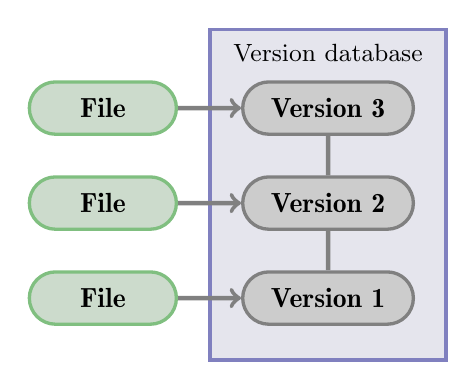
\begin{tikzpicture}[
                file/.style={
                    rounded rectangle,
                    minimum size=6mm,
                    very thick,
                    draw=green!50!black!50,
                    fill=green!30!black!20,
                    inner sep=6pt,
                    text width=14mm,
                    text centered,
                    font=\bf
                },
                version/.style={
                    rounded rectangle,
                    minimum size=6mm,
                    very thick,
                    draw=black!50,
                    fill=black!20,
                    inner sep=6pt,
                    text width=17mm,
                    text centered,
                    font=\bf
                },
                point/.style={coordinate},
                path/.style={ultra thick,draw=black!50,rounded corners},
                ]
            \draw [very thick, draw=blue!50!black!50, fill=blue!30!black!10]
            (-.5,1) rectangle
            (2.5,-3.2);
            \node at (1, .7) {\small Version database};
            \node (v3) [version] at (1,0) {Version 3};
            \node (v2) [version, below=5mm of v3] {Version 2};
            \node (v1) [version, below=5mm of v2] {Version 1};
            \draw [path] (v3) -- (v2);
            \draw [path] (v2) -- (v1);
            \node<5> (f) [file, left=8mm of v3] {File};
            \draw<5> [path, ->] (f) -- (v3);
            \node<6> (f) [file, left=8mm of v2] {File};
            \draw<6> [path, ->] (f) -- (v2);
            \node<7> (f) [file, left=8mm of v1] {File};
            \draw<7> [path, ->] (f) -- (v1);
            \end{tikzpicture}}
        \end{column}
    \end{columns}
\end{frame}

\begin{frame}[t]
    \frametitle{Version control: use case}
    \begin{block}{Collaboration through e-mail:}
    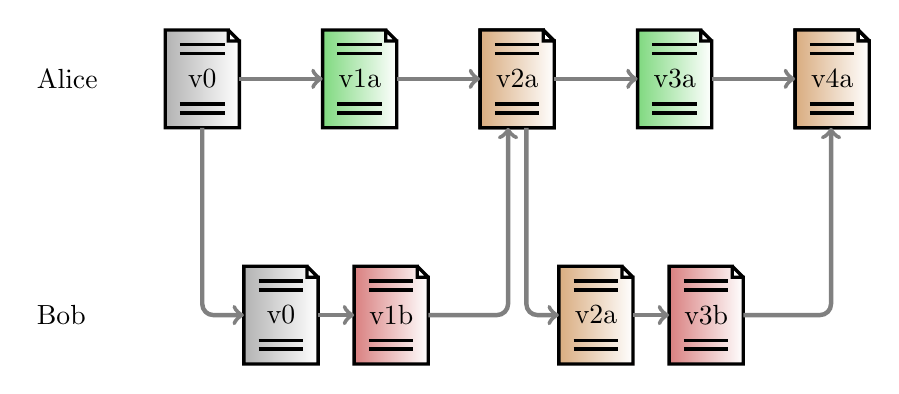
\begin{tikzpicture}[
                path/.style={ultra thick,draw=black!50,rounded corners},
            ]
            \node<1-10> [text width=12mm, minimum height=13mm] at (0.5,1.5) {Alice};
            \node [text width=12mm, minimum height=13mm] at (0.5,-1.5) {Bob};
            \node (v0) [doctype,draw,very thick,color=black, left
            color=black!30, right color=white,minimum height=12mm,minimum
            width=9mm] at (2,1.5) {v0};
            \node<2-> (v0c) [doctype,draw,very thick,color=black, left
            color=black!30, right color=white,minimum height=12mm,minimum
            width=9mm] at (3,-1.5) {v0};
            \node<3-> (v1a) [doctype,draw,very thick,color=black, left
            color=green!70!black!50, right color=white,minimum height=12mm,minimum
            width=9mm] at (4,1.5) {v1a};
            \node<3-> (v1b) [doctype,draw,very thick,color=black, left
            color=red!70!black!50, right color=white,minimum height=12mm,minimum
            width=9mm] at (4.4,-1.5) {v1b};
            \node<4-> (v1bc) [doctype,draw,very thick,color=black, left
            color=red!70!black!50, right color=white,minimum height=12mm,minimum
            width=9mm] at (6,1.5) {v1b};
            \node<5-> (v2a) [doctype,draw,very thick,color=black, left
            color=orange!70!black!50, right color=white,minimum height=12mm,minimum
            width=9mm] at (6,1.5) {v2a};
            \node<6-> (v2ac) [doctype,draw,very thick,color=black, left
            color=orange!70!black!50, right color=white,minimum height=12mm,minimum
            width=9mm] at (7,-1.5) {v2a};
            \node<7-> (v3a) [doctype,draw,very thick,color=black, left
            color=green!70!black!50, right color=white,minimum height=12mm,minimum
            width=9mm] at (8,1.5) {v3a};
            \node<7-> (v3b) [doctype,draw,very thick,color=black, left
            color=red!70!black!50, right color=white,minimum height=12mm,minimum
            width=9mm] at (8.4,-1.5) {v3b};
            \node<8-> (v3bc) [doctype,draw,very thick,color=black, left
            color=red!70!black!50, right color=white,minimum height=12mm,minimum
            width=9mm] at (10,1.5) {v3b};
            \node<9-> (v4a) [doctype,draw,very thick,color=black, left
            color=orange!70!black!50, right color=white,minimum height=12mm,minimum
            width=9mm] at (10,1.5) {v4a};

            \draw<3-9> [path, ->] (v0) -- (v1a);
            \draw<5-9> [path, ->] (v1a) -- (v2a);
            \draw<7-9> [path, ->] (v2a) -- (v3a);
            \draw<9> [path, ->] (v3a) -- (v4a);

            \draw<2-9> [path, ->] (v0) |- (v0c);
            \draw<3-9> [path, ->] (v0c) -- (v1b);
            \draw<4-9> [path, ->] (v1b) -| ([xshift=-16pt]v1bc);
            \draw<6-9> [path, ->] ([xshift=16pt]v2a) |- (v2ac);
            \draw<7-9> [path, ->] (v2ac) -- (v3b);
            \draw<8-9> [path, ->] (v3b) -| ([xshift=-2pt]v3bc);
    \end{tikzpicture}
    \end{block}
\end{frame}

\begin{frame}[t]
    \frametitle{Version control: use case}
    \begin{block}{Collaboration through central data storage:}
    \begin{tikzpicture}[
                path/.style={ultra thick,draw=black!50,rounded corners},
                lock/.style={ultra thick,draw=red!50,rounded corners},
            ]
            \node<1-9> [text width=12mm, minimum height=13mm] at (0.5,1.5) {Alice};
            \node [text width=12mm, minimum height=13mm] at (0.5,-1.5) {Bob};
            \node [text width=12mm] at (0.5,0) {Server};
            % Server
            \node (v0) [doctype,draw,very thick,color=black, left
            color=black!30, right color=white,minimum height=12mm,minimum
            width=9mm] at (2,0) {v0};
            \node<4-8> (v1b) [doctype,draw,very thick,color=black, left
            color=black!30, right color=white,minimum height=12mm,minimum
            width=9mm] at (6,0) {v1b};
            \node<7-> (v2a) [doctype,draw,very thick,color=black, left
            color=black!30, right color=white,minimum height=12mm,minimum
            width=9mm] at (10,0) {v2a};

            \node<9> (v0) [doctype,draw,very thick,color=black!50, left
            color=black!10, right color=white,minimum height=12mm,minimum
            width=9mm] at (2,0) {v0};
            \node<9> (v1b) [doctype,draw,very thick,color=black!50, left
            color=black!10, right color=white,minimum height=12mm,minimum
            width=9mm] at (6,0) {v1b};

            %Alice
            \node (a1) at (2,1.5) {};
            \node<8> at (4,1.5) {\includegraphics[width=10mm]{images/coffee.png}};
            \node<5-8> (v1a) [doctype,draw,very thick,color=black, left
            color=green!70!black!50, right color=white,minimum height=12mm,minimum
            width=9mm] at (8,1.5) {v1a};

            %Bob
            \node (b1) at (6,-1.5) {};
            \node<2-8> (v0b) [doctype,draw,very thick,color=black, left
            color=red!70!black!50, right color=white,minimum height=12mm,minimum
            width=9mm] at (4,-1.5) {v0b};
            \node<8> at (8,-1.5) {\includegraphics[width=10mm]{images/coffee.png}};

            \draw<3-8> [path, ->] (v0) -- node {\textcolor{red}{\textbf{X}}} (a1);
            \draw<2-8> [path, ->] ([xshift=-16pt]v0) |- ([yshift=-16pt]v0b);
            \draw<3-8> [lock, ->] ([yshift=8pt]v0b) -| ([xshift=8pt]v0);
            \node<3-8> at (2.7,-1.2) {LOCK};
            \draw<4-8> [path, ->] (v0b) -| ([xshift=-16pt]v1b);
            \draw<6-8> [path, ->] (v1b) -- node {\textcolor{red}{\textbf{X}}} (b1);

            \draw<5-8> [path, ->] ([xshift=-16pt]v1b) |- ([yshift=16pt]v1a);
            \draw<6-8> [lock, <-] ([xshift=6pt]v1b) |- ([yshift=-8pt]v1a);
            \node<6-8> at (6.7,1.2) {LOCK};
            \draw<7-8> [path, ->] (v1a) -| (v2a);
    \end{tikzpicture}
    \end{block}
\end{frame}

\begin{frame}[t]
    \frametitle{Version control: use case}
    \begin{block}{Collaboration with version control system:}
    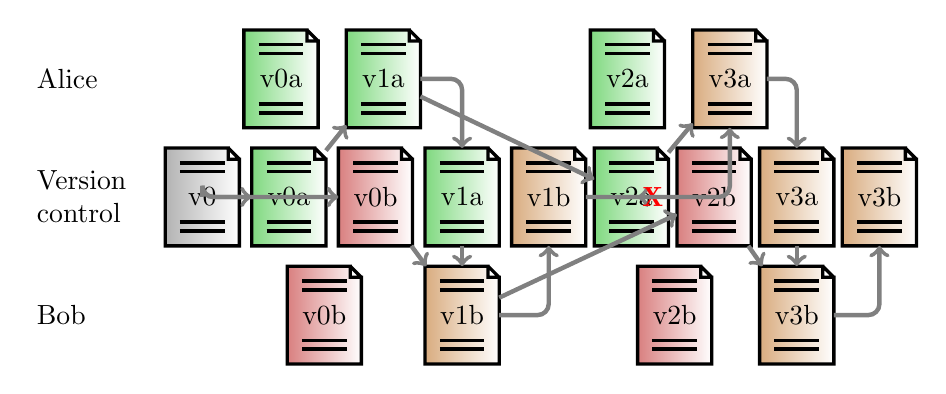
\begin{tikzpicture}[
                path/.style={ultra thick,draw=black!50,rounded corners},
                point/.style={coordinate},
            ]
            \node [text width=12mm, minimum height=13mm] at (0.5,1.5) {Alice};
            \node [text width=12mm, minimum height=13mm] at (0.5,-1.5) {Bob};
            \node [text width=12mm] at (0.5,0) {Version control};
            % Server
            \node (v0) [doctype,draw,very thick,color=black, left
            color=black!30, right color=white,minimum height=12mm,minimum
            width=9mm] at (2,0) {v0};
            \node<3-> (v1) [doctype,draw,very thick,color=black, left
            color=green!70!black!50, right color=white,minimum height=12mm,minimum
            width=9mm] at (5.3,0) {v1a};
            \node<5-> (v2) [doctype,draw,very thick,color=black, left
            color=orange!70!black!50, right color=white,minimum height=12mm,minimum
            width=9mm] at (6.4,0) {v1b};
            \node<9-> (v3) [doctype,draw,very thick,color=black, left
            color=orange!70!black!50, right color=white,minimum height=12mm,minimum
            width=9mm] at (9.55,0) {v3a};
            \node<11-> (v4) [doctype,draw,very thick,color=black, left
            color=orange!70!black!50, right color=white,minimum height=12mm,minimum
            width=9mm] at (10.6,0) {v3b};

            \node (s1) at (7.4,0) {};

            %Alice
            \node<2-11> (v0a) [doctype,draw,very thick,color=black, left
            color=green!70!black!50, right color=white,minimum height=12mm,minimum
            width=9mm] at (3,1.5) {v0a};
            \node<2-11> (v1a) [doctype,draw,very thick,color=black, left
            color=green!70!black!50, right color=white,minimum height=12mm,minimum
            width=9mm] at (4.3,1.5) {v1a};
            \node<6-11> (v2a) [doctype,draw,very thick,color=black, left
            color=green!70!black!50, right color=white,minimum height=12mm,minimum
            width=9mm] at (7.4,1.5) {v2a};
            \node<8-11> (v3a) [doctype,draw,very thick,color=black, left
            color=orange!70!black!50, right color=white,minimum height=12mm,minimum
            width=9mm] at (8.7,1.5) {v3a};

            \node<12> (v0a) [doctype,draw,very thick,color=black, left
            color=green!70!black!50, right color=white,minimum height=12mm,minimum
            width=9mm] at (3.1,0) {v0a};
            \node<12> (v2a) [doctype,draw,very thick,color=black, left
            color=green!70!black!50, right color=white,minimum height=12mm,minimum
            width=9mm] at (7.45,0) {v2a};

            %Bob
            \node<2-11> (v0b) [doctype,draw,very thick,color=black, left
            color=red!70!black!50, right color=white,minimum height=12mm,minimum
            width=9mm] at (3.55,-1.5) {v0b};
            \node<4-11> (v1b) [doctype,draw,very thick,color=black, left
            color=orange!70!black!50, right color=white,minimum height=12mm,minimum
            width=9mm] at (5.3,-1.5) {v1b};
            \node<6-11> (v2b) [doctype,draw,very thick,color=black, left
            color=red!70!black!50, right color=white,minimum height=12mm,minimum
            width=9mm] at (8,-1.5) {v2b};
            \node<10-11> (v3b) [doctype,draw,very thick,color=black, left
            color=orange!70!black!50, right color=white,minimum height=12mm,minimum
            width=9mm] at (9.55,-1.5) {v3b};

            \node<12> (v0b) [doctype,draw,very thick,color=black, left
            color=red!70!black!50, right color=white,minimum height=12mm,minimum
            width=9mm] at (4.2,0) {v0b};
            \node<12> (v2b) [doctype,draw,very thick,color=black, left
            color=red!70!black!50, right color=white,minimum height=12mm,minimum
            width=9mm] at (8.5,0) {v2b};

            %Alice
            \draw<2-11> [path, ->] (v0) |- (v0a);
            \draw<2-11> [path, ->] (v0a) -- (v1a);
            \draw<3-11> [path, ->] (v1a) -| (v1);
            \draw<6-11> [path, ->] (v1a) -- (v2a);
            \draw<7-11> [path, ->] (v2a) -- node {\textcolor{red}{\textbf{X}}} (s1);
            \draw<8-11> [path, ->] (v2) -| (v3a);
            \draw<8-11> [path, ->] (v2a) -- (v3a);
            \draw<9-11> [path, ->] (v3a) -| (v3);

            %Bob
            \draw<2-11> [path, ->] (v0) |- (v0b);
            \draw<4-11> [path, ->] (v0b) -- (v1b);
            \draw<4-11> [path, ->] (v1) -- (v1b);
            \draw<5-11> [path, ->] (v1b) -| (v2);
            \draw<6-11> [path, ->] (v1b) -- (v2b);
            \draw<10-11> [path, ->] (v2b) -- (v3b);
            \draw<10-11> [path, ->] (v3) -- (v3b);
            \draw<11> [path, ->] (v3b) -| (v4);


    \end{tikzpicture}
    \end{block}
\end{frame}

\begin{frame}
    \frametitle{Version control: a secret language?}
    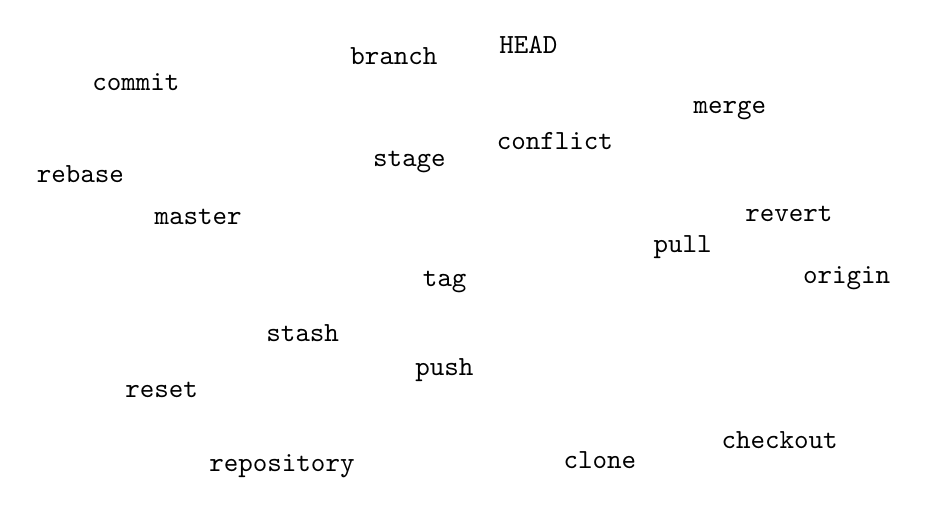
\begin{tikzpicture}
        \node at (7.17891069,0.15999506) {\texttt{clone}};
        \node at (1.28720694,4.96402701) {\texttt{commit}};
        \node at (5.20508947,1.30920676) {\texttt{push}};
        \node at (8.2323718 ,2.87233088) {\texttt{pull}};
        \node at (5.20847529,2.42919482) {\texttt{tag}};
        \node at (4.56512354,5.29905495) {\texttt{branch}};
        \node at (8.82965476,4.60563145) {\texttt{merge}};
        \node at (9.46412647,0.4158012 ) {\texttt{checkout}};
        \node at (9.58172758,3.29374652) {\texttt{revert}};
        \node at (0.58258464,3.7927869 ) {\texttt{rebase}};
        \node at (1.61278255,1.04671331) {\texttt{reset}};
        \node at (3.14283779,0.08804959) {\texttt{repository}};
        \node at (2.07678489,3.25027926) {\texttt{master}};
        \node at (6.27224224,5.42899499) {\texttt{HEAD}};
        \node at (10.3150507,2.47376899) {\texttt{origin}};
        \node at (4.76038417,3.94133488) {\texttt{stage}};
        \node at (3.40436500,1.77992114) {\texttt{stash}};
        \node at (6.60742742,4.21405916) {\texttt{conflict}};
    \end{tikzpicture}
\end{frame}

\section{git}

\begin{frame}
    \frametitle{What is git?}
    \begin{itemize}
        \item Built as version control tool for the Linux kernel
            \begin{itemize}
                \item Built for speed
                \item Designed for large projects
                \item Designed for many collaborators
            \end{itemize}
        \item Distributed version control system
            \begin{itemize}
                \item Fast: all operations are performed locally
                \item No backup needed: every copy holds the full database
                \item No network connection needed
            \end{itemize}
        \item Records a snapshot for each version of files
            \begin{itemize}
                \item Files can be reverted to any state
                \item Allows working on different versions simultaneously
            \end{itemize}
        \item Works best with line based text files
            \begin{itemize}
                \item Source code etc.
            \end{itemize}
    \end{itemize}
\end{frame}

%\begin{frame}
%    \frametitle{Repository structure}
%\end{frame}

\begin{frame}[t,squeeze]
    \frametitle{Basic commands}
    \only<1-7,9-12>{\vspace{-7mm}
        \small
        \begin{columns}[T]
            \begin{column}{.33\linewidth}
                \uncover<2->{\begin{block}{Create repository}
                        \texttt{git init}
                \end{block}}
                \vspace{-1.2mm}
                \uncover<2->{\begin{block}{Add files}
                        \texttt{git add <file>}
                \end{block}}
                \vspace{-1.2mm}
                \uncover<11->{\begin{block}{Revert changes}
                        \texttt{git reset ---hard}
                \end{block}}
                \vspace{-1.2mm}
                \uncover<7->{\begin{block}{Show status}
                        \texttt{git status}
                \end{block}}
                \vspace{-1.2mm}
                \uncover<6->{\begin{block}{Stash changes}
                        \texttt{git stash}\\
                        \texttt{git stash list}\\
                        \texttt{git stash apply}
                \end{block}}
            \end{column}
            \begin{column}{.66\linewidth}
                \uncover<3->{\begin{block}{Commit}
                        \texttt{git commit -m "Commit message."}\\
                        Commit all changes:\\
                        \texttt{git commit -a -m "Commit message."}
                \end{block}}
                \vspace{-2mm}
                \begin{columns}
                    \begin{column}{.45\linewidth}
                        \uncover<4->{\begin{block}{Create branch}
                                \texttt{git branch <branch name>}
                        \end{block}}
                    \end{column}
                    \begin{column}{.45\linewidth}
                        \uncover<12->{\begin{block}{Merge}
                                \texttt{git merge <other branch>}
                        \end{block}}
                    \end{column}
                \end{columns}
                \vspace{-1mm}
                \uncover<10->{\begin{block}{Create tag}
                        \texttt{git tag -a <tag> -m"Description"}\\
                        \texttt{git tag}
                \end{block}}
                \vspace{-1.5mm}
                \uncover<5->{\begin{block}{Switch version}
                        \texttt{git checkout <branch>}\\
                        \texttt{git checkout <tag>}\\
                        \texttt{git checkout <version>}
                \end{block}}
            \end{column}
    \end{columns}}
    \only<8>{\begin{center}\begin{tikzpicture}
            \node [rectangle, text width=20mm, minimum height=11mm, draw=none, fill=red!50!black!50]
            at (0,6) {Working directory};
            \node [rectangle, text width=20mm, minimum height=11mm, draw=none, fill=orange!50!black!50]
            at (4,6) {Staging area};
            \node [rectangle, text width=20mm, minimum height=11mm, draw=none, fill=green!50!black!50]
            at (8,6) {Repository};
            \draw [ultra thick, draw=red!75!black] (0,0) -- (0,5);
            \draw [ultra thick, draw=orange!75!black] (4,0) -- (4,5);
            \draw [ultra thick, draw=green!75!black] (8,0) -- (8,5);
        \node[scalearrow,
              scalearrow width=12mm,
              minimum height = 40mm,
              rotate = 90,
          fill=red!50] at (2, 4.0) {};
          \node at (2,4.0) {add};
        \node[scalearrow,
              scalearrow width=12mm,
              minimum height = 40mm,
              rotate = 90,
          fill=green!50] at (6, 2.5) {};
          \node at (6,2.5) {commit};
        \node[scalearrow,
              scalearrow width=12mm,
              minimum height = 80mm,
              rotate = -90,
          fill=blue!50] at (4, 1.0) {};
          \node at (4,1.0) {checkout};
        \end{tikzpicture}
    \end{center}}
\end{frame}

%\begin{frame}
%    \frametitle{Tools}
%    \begin{columns}
%        \begin{column}{.5\linewidth}
%            \begin{block}{GUI}
%                \begin{itemize}
%                    \item 
%                \end{itemize}
%            \end{block}
%            \begin{block}{Integration into operating system}
%                \begin{itemize}
%                    \item Tortoise git
%                \end{itemize}
%            \end{block}
%        \end{column}
%        \begin{column}{.5\linewidth}
%            \begin{block}{Text editors}
%                \begin{itemize}
%                    \item Sublime
%                    \item Vim
%                \end{itemize}
%            \end{block}
%        \end{column}
%    \end{columns}
%\end{frame}

%\section{Links}

\begin{frame}[t]
    %\frametitle{\texttt{git}}
    \vspace{20mm}
    \includegraphics[width=\textwidth]{images/Git-Logo-2Color.png}
\end{frame}

%\section{GitHub}
%
%\begin{frame}
%    \frametitle{GitHub}
%    \begin{itemize}
%        \item Web-based git hosting service
%            \begin{itemize}
%                \item Public repositories for free
%                \item Private repositories (monthly fee)
%            \end{itemize}
%        \item Issue tracking
%    \end{itemize}
%\end{frame}

%\begin{frame}
%    \frametitle{Local copy - staging area - repository}
%\end{frame}

\begin{frame}
    \frametitle{Links}
    \textbf{git}: \texttt{\url{http://git-scm.com/}}\\
    \textbf{GitHub}: \texttt{\url{http://github.com}}\\
    \medskip
    GUIs:
    \begin{itemize}
        \item \textbf{TortoiseGit}: \texttt{\url{https://code.google.com/p/tortoisegit/}}
        \item \textbf{SmartGit}: \texttt{\url{http://www.syntevo.com/smartgit/}}
    \end{itemize}
    \medskip
    Editors:
    \begin{itemize}
        \item \textbf{Vim}: \texttt{\url{http://www.vim.org/}}
        \item GitGutter for vim: \texttt{\url{https://github.com/airblade/vim-gitgutter}}
        \item \textbf{Sublime}: \texttt{\url{http://www.sublimetext.com/}}
        \item GitGutter for sublime: \texttt{\url{https://github.com/jisaacks/GitGutter}}
    \end{itemize}
\end{frame}

% LAST SLIDE %%%%%%%%%%%%%%%%%%%%%%%%%%%%%%%%%%%%%%%%%%%%%%%%%%%%%%%%%%%%%%%%%
%\setbeamertemplate{footline}[default]
%\begin{frame}
%    \vspace{-4mm}
%    \mbox{\hspace{-8mm}\includegraphics[width=\textwidth+33mm]{images/IMG_4773.JPG}}\\
%\end{frame}

%\addtocounter{framenumber}{-1}
%\setbeamertemplate{footline}[default]
%\setbeamertemplate{headerline}[default]
%
%\begin{frame}[t]
%    \frametitle{Future value function (SDDP)}
%    \vspace{-5ex}
%    \includegraphics[width=\textwidth]{gnuplot/hyperplanes.pdf}
%\end{frame}

\end{document}
